%=======================================================================
% SM 4/2017
% Master's thesis Report IISER Thiruvananthapuram
% Investigations of SpinTaylorF2
%=======================================================================

\chapter{Bounds on astrophysical parameters}

In the previous chapter, we observed that the total SNR of the SpinTaylorF2
waveform is primarily divided between the $m=0$ and $m=2$ sidebands for a
large fraction of the spin-precession parameter space. Further, these two
sidebands dominate in almost complimentary regions of $(\theta_J, \kappa)$
parameter space: the $m=0$ mode appears to dominate for mildly precessing
systems, whereas $m=0$ mode dominates over the $m=2$ mode for strongly
precessing, edge-on binaries.

The fact that two sidebands capture most of the SNR over a large, but
complimentary regions of the parameter space, naturally leads to 3 possible
scenarios---the first two, where either $m=0$ or $m=2$ mode dominates over the
other, and the third, where both of these modes have comparable contribution
to the total SNR. In the sections below, we identify three regions $(\theta_J,
\kappa)$ space associated with strongly precessing, moderately precessing, and
mildly (non)-precessing systems, depending on the relative contribution of the
two sidebands to the full waveform.

\section{Partitioning the spin-precession parameter space}

\begin{figure}[!tp]
\centering
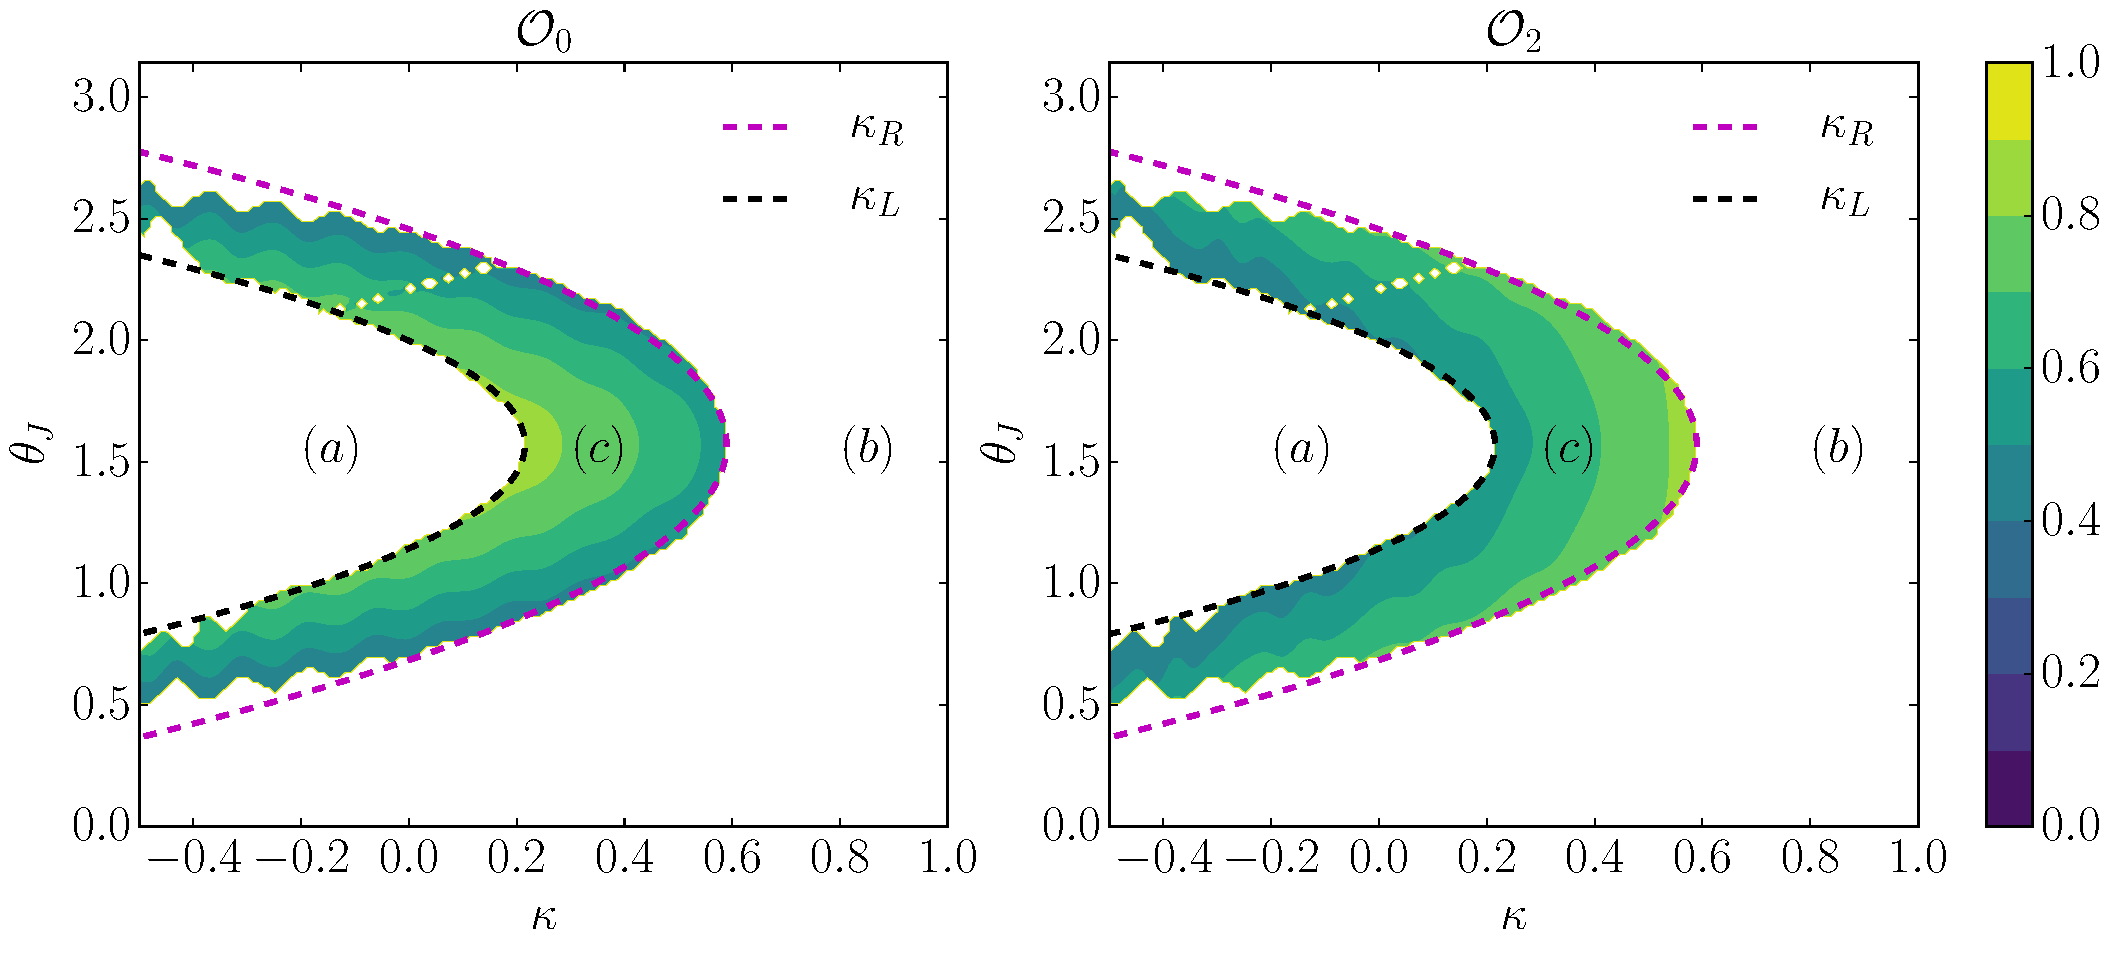
\includegraphics[width=0.8\linewidth]{images/OVLP_cut.pdf}
\caption{\small{Comparison of the overlaps, ${\cal{O}}_2$ and ${\cal{O}}_0$
for ${\cal{O}}_2, ~{\cal{O}}_0 > 0.4$ in the $(\theta_J, \kappa)$ parameter
space, for $m_{1}=14M_{\odot}$ and $\chi_1=0.8$. The three regions: region~(a)
where ${\cal{O}}_0 - {\cal{O}}_2 > 0.3$, region~(b) where ${\cal{O}}_2 -
{\cal{O}}_0 > 0.3$, and regions~(c) where $|{\cal{O}}_2-{\cal{O}}_0|< 0.3$.}}
\label{FIG:OVLP_cut_regions}
\end{figure}

We identified three regions in the $(\theta_J, \kappa)$ parameter space:
region~(a) where ${\cal{O}}_0$ is dominant $({\cal{O}}_0 - {\cal{O}}_2 >
0.3)$, region~(b) where ${\cal{O}}_2$ is dominant $({\cal{O}}_2 - {\cal{O}}_0
> 0.3)$, and finally, region~(c) where ${\cal O}_2$ and ${\cal O}_0$ are
comparable $(|{\cal{O}}_2-{\cal{O}}_0|< 0.3)$ to each other. We also enforced
the condition that both ${\cal O}_2$ and ${\cal O}_0$ are greater than or
equal to $0.4$ in all regions, in order to ensure both the sidebands are above
above the detectable threshold. The results is shown in
Fig.~\ref{FIG:OVLP_cut_regions}, which shows the three regions in the
$(\theta_J,\kappa)$ space for an NSBH system with BH mass $m_{1}=14 M_\odot$,
$\chi_1=0.8$, $\psi_J=0.001$ and $\alpha_0 =0.001$.


We approximated the boundaries of region~(c) by using two parabolas symmetric
around $\theta_J=\pi/2$, as functions of $\eta$ and $\chi_1$:
\begin{equation}
\kappa(\eta, \chi_1) = \kappa_{0}(\eta, \chi_1) - C(\eta, \chi_1)(\theta_J-\pi/2)^2, 
\label{EQ:boundary_region}
\end{equation}
where $\kappa_{0}(\eta, \chi_1)$ and $C(\eta, \chi_1)$ is given by
\begin{align}
\begin{split}
\kappa_{0a}(\eta, \chi_{1})~&\approx  (145.83 \chi_{1} - 155.92)\, \eta^2 -
(1.10 \chi_{1} + 0.16)\, \eta+ 0.08 \, \chi_{1}+0.50,\\
\kappa_{0b}(\eta, \chi_{1})~&\approx (48.98\chi_{1} - 57.13) \,\eta^2 +
(1.96{\chi_{1}}-2.39)\, \eta - 0.09 \, \chi_{1} +0.82,
\label{EQ:kappa_boundary}
\end{split}
\end{align}
\vspace{-10mm}
\begin{align}
\begin{split}
C_{a}(\eta, \chi_{1})~&\approx  (-6.23{\chi_{1}} + 10.47)\,
\eta +  0.01\, \chi_{1}+ 0.72,\\
C_{b}(\eta, \chi_{1})~&\approx  (-8.37{\chi_{1}} + 10.62)\, \eta +  0.10\,
\chi_{1}+ 0.30,
\label{EQ:phi_boundary}
\end{split}
\end{align}
where the subscript `$a$' and `$b$' represent the boundaries of region~(a) and
region~(b) with region~(c), respectively. We obtained the expressions for
$\kappa_{0}(\eta, \chi_1)$ and $C(\eta, \chi_1)$ by fitting a quadratic
function to the points on the boundaries of these regions over a range of
values for $\eta$ and $\chi_1$ ($0.08 < \eta < 0.24$ and $0 < \chi_1 < 1$).
As the extent of precession increases (i.e., for higher values of BH
mass/spin), the inner boundary that separates region~(b) and region~(c) shifts
to higher values of $\kappa$, since the contribution of the $m=0$ mode
increases. These fits, therefore, can used to probe the extent of precession
in the system, depending on where the system lies in the $(\theta_J,
\kappa)$ space.

\section{Upper bound on $\kappa$}

Figure ~\ref{FIG:OVLP_cut_regions} immediately suggests that there exists an
upper bound on the spin-alignment parameter $\kappa$ for strongly and
moderately precessing systems, i.e., systems in in region~(a) and region~(c).
In the case where the $m=0$ sideband has a significantly larger SNR than
$m=2$, we can assert that the system lies in region~(a) in
Fig.~\ref{FIG:OVLP_cut_regions}, which implies that the system is strongly
precessing. We can then use
Eqs.~(\ref{EQ:boundary_region})--(\ref{EQ:phi_boundary}), given we are able to
estimate $\eta$ using the total and the chirp mass of the binary, to bound the
spin orientation $\kappa$, depending on the BH spin.


For example, in Fig.~\ref{FIG:kappa_max_bounds} we show the variation in the
upper bound on $\kappa$ with $\chi_1$ (left) and $\eta$ (right), for two the
regions (a) and (c), corresponding to strongly precessing and moderately
precessing systems, respectively. Each of these features observed in
Fig.~\ref{FIG:kappa_max_bounds} can be explained by taking into account the
effect of $\kappa, \chi_1$ and $\eta$ on the extent of precession in the
system.

We observe that with increasing BH spin (for $m_1=14.0\,M_{\odot}$), the
maximum allowed value of $\kappa$ also increases. This is consistent with the
fact that for very high values of spin, even moderately misaligned systems can
show high amount of spin-induced precession. Notably, even for $\chi_1=1$
(highest possible BH spin), we observe that there exists an upper bound on
$\kappa \leq 0.64$ for moderately precessing systems in region~(c), and
$\kappa \leq 0.41$ for systems that are strongly precessing, i.e. those in
region~(a). Therefore, even we if do not have an esimate of the BH spin, we
see that we can significantly constrain the possible values of the spin-
alignment parameter $\kappa$.

Further, we observe that for lower values of $\eta$, i.e. high BH masses, the
upper bound on $\kappa$ increases (for $\chi_1=0.8$). This is again consistent
with the fact that high mass asymmetry can compensate for moderately aligned
BH spin, to result in the same amount of precession. In summary, the upper
bound on $\kappa$ increases with both BH mass and BH spin. In practice, this
could be useful, since, even for highest possible BH spin $(\chi_1=1.0)$ and
relatively high BH mass $(m_1=100)$, we found that the maximum possible value
of $\kappa$ for a moderately precessing system is restricted to $(\kappa <
0.72)$.

\begin{figure}[!http]
\centering
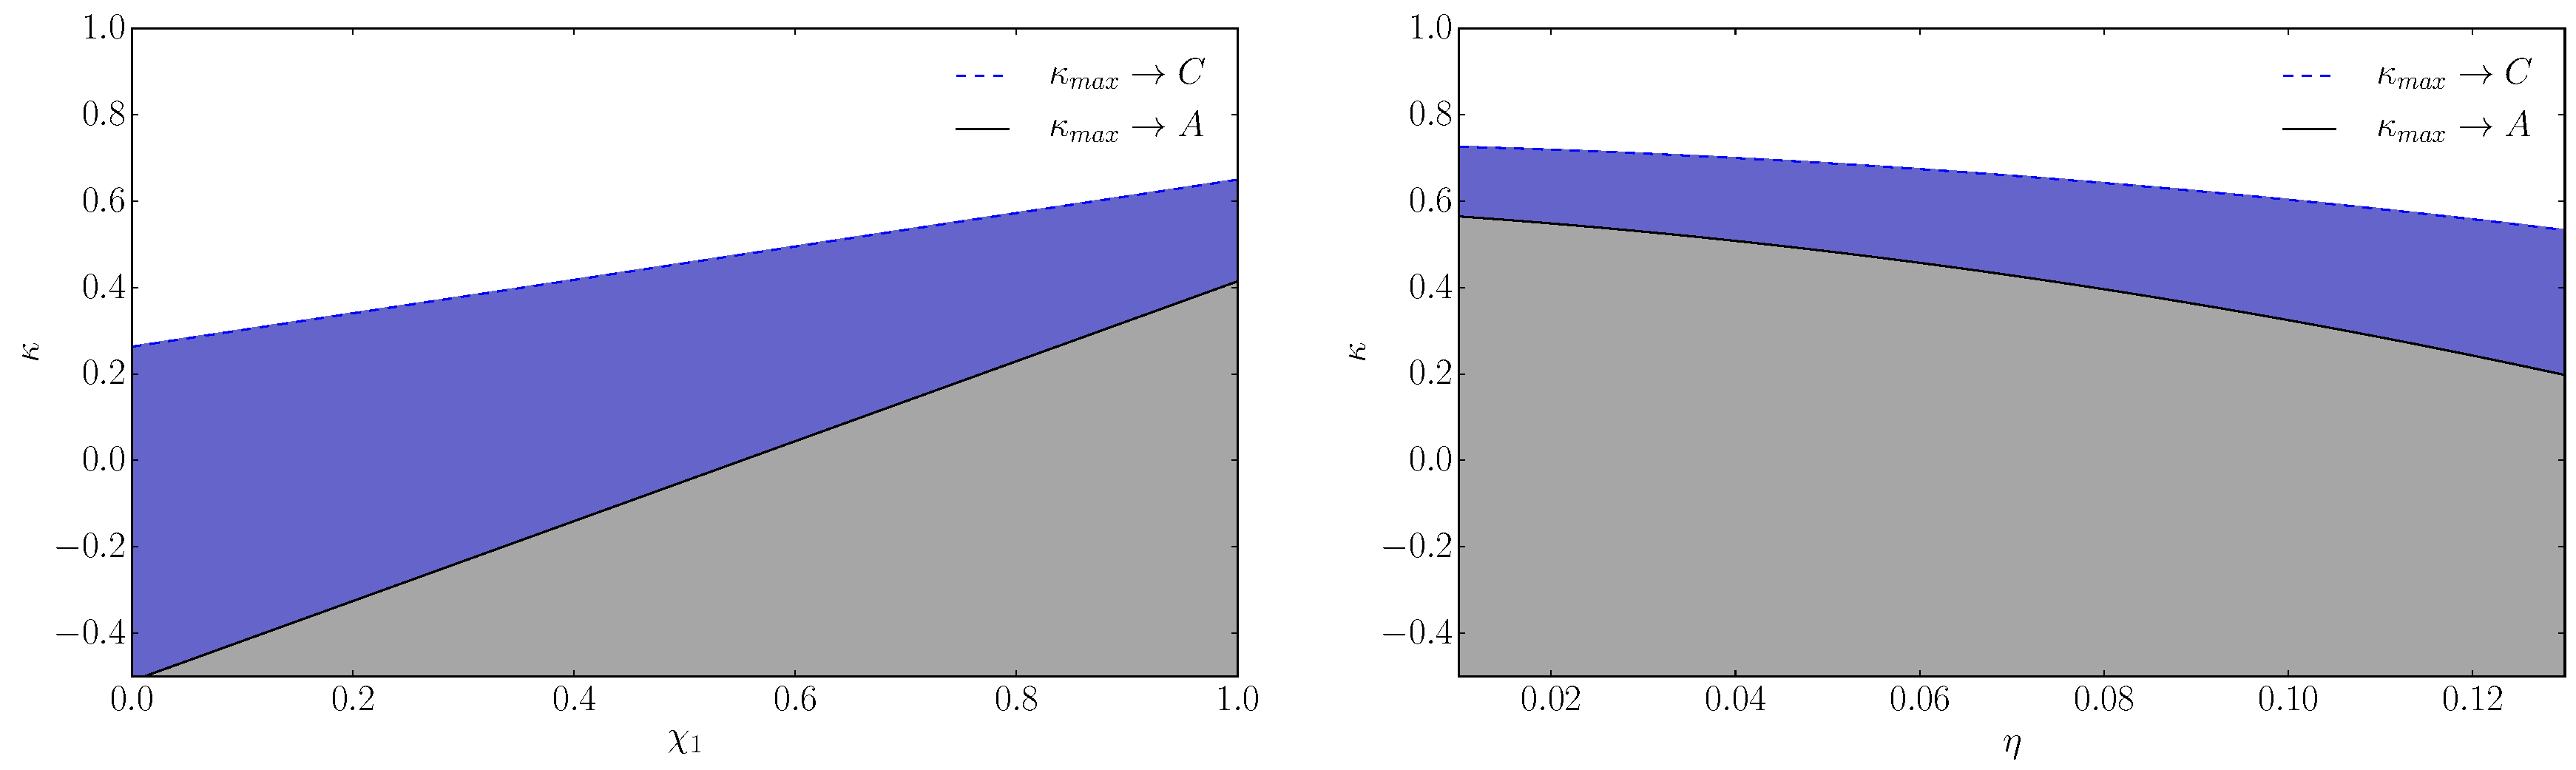
\includegraphics[width=1.0\linewidth]{images/kappa_max_bound.pdf} 
\caption{\small{The dashed line corresponds to the maximum value of $\kappa$ for
    a strongly precessing system ($m_1 = 14 M_{\odot}, m_2 = 1.4 M_{\odot}$),
    i.e, region~(a) and moderately precessing systems that lie in region~(b)
    in Fig.~\ref{FIG:OVLP_cut_regions}.}}
\label{FIG:kappa_max_bounds}
\end{figure}
